\section{Implementation and evaluation}
%03 12 2014
\subsection{Dataset}
Physical activity of a subject was assessed during daily life by mean of the SenseWear Armband and SenseWear Mini Armband activity monitors. 
These devices combine an accelerometer with different physiological sensors (a heat flux sensor, a galvanic skin response sensor, 
a skin temperature sensor, and a near-body ambient temperature sensor).  Together with demographic characteristics, such as gender, 
age, height and weight, energy expenditure (EE) and metabolic equivalent of task (MET) were estimated using proprietary algorithms 
developed by the manufacturer. Moreover, information about the sleeping status of a subject (0=awake, 1=sleeping) is also provided. 
The SenseWear Armband has been shown to be valid both in field~\cite{Colbert_2011,Mackey_2011} and in laboratory 
studies~\cite{Furlanetto_2010,Hill_2010,Cavalheri_2011}.
\par Data from 1001 COPD patients (65\% men; age, 67 years; $FEV_{1}$, 49\% predicted; BMI, 25.8) were recorded across 10 different countries. Subjects wore the sensor both during day time and night time so that continuous, non-scripted activities were recorded in a natural environment with 1 minute resolution. 
A minimum of 4 days (2 weekdays + Saturday + Sunday) was considered acceptable to include a patient in the analysis~\cite{Watz_2009}, with the device 
being used for at least 22 hours per day. 
%Since data presents intrinsic variability due to different
%awakening and sleeping times of the subjects we tried
%to minimize this synchronizing the days according to the
%morning awakening points, considered as the time instant
%after the longest period of sleep. Data before the awakening
%point were discarded from the analysis.
In order to minimize the intrinsic variability of data 
%that is due to different subjects' awake and sleep periods. Data prior to the awakening point was discarded from the analysis, 
recorded days were synchronized according to the morning time instants after the longest period of sleep (awakening points). Data prior to the awakening point was discarded from the analysis.
\par The median number of days analyzed per patient was 6 (4 weekdays - 2 weekend days), resulting in a total of 5846 valid PA days assessed, of which 3916 (67\%) were weekdays and 1930 (33\%) weekend days.
% (see Table~\ref{table:Table1})
A median of 982 minutes were analyzed per patient each day (992 weekdays - 961 weekend days).
%The median number of valid synchronized days per patients was 6 (4 weekdays - 2 weekend days) days, resulting in a total of 798 valid PA days, of which 536 (\%67.17) were weekdays and 262 (\%32.83).% (see Table~\ref{table:Table2}). 
%In 5 days the awakening point was not found and then those days were discarded.
%The median number of minutes assessed per day was 1425 when the full days were taken into account, 972 considering only the awake hours. 
Ethics Board approval was obtained from the local ethics committees, and written informed consent was provided by participants.\\

%%%%%%%%%%%%%%%%%%%%%%%%%%%%%	TABLE STATISTICS DATA		%%%%%%%%%%%%%%%%
% COPD + HEALTHY
% not sync
%\begin{table}[H!]
%\centering
%\begin{tabular}{|c|c|c|c|}
%\hline
% & All days & Weekends & Weekdays \\
%\hline
%Number of days & 804.000 & 266.000 & 538.0 \\
%\hline
%Percentage & - & 33.085 & 66.9 \\
%\hline
%Median days & 6.000 & 2.000 & 4.0 \\
%\hline
%Median minutes & 1425.000 & 1425.000 & 1425.0 \\
%\hline
%\end{tabular}
%\caption{Assessment day statistics}
%\label{table:Table1}
%\end{table}
%
% sync
%\begin{table}[H!]
%\centering
%\begin{tabular}{|c|c|c|c|}
%\hline
% & All days & Weekends & Weekdays \\
%\hline
%Number of days & 799.000 & 263.000 & 536.0 \\
%\hline
%Percentage & - & 33.085 & 67.1 \\
%\hline
%Median days & 6.000 & 2.000 & 4.0 \\
%\hline
%Median minutes & 972.000 & 946.000 & 983.5 \\
%\hline
%\end{tabular}
%\caption{Assessment sync day statistics}
%\label{table:Table2}
%\end{table}

% 977 COPD
% not sync
%\begin{table}[H!]
%\centering
%\begin{tabular}{|c|c|c|c|}
%\hline
% & All days & Weekends & Weekdays \\
%\hline
%Number of days & 5938.000 & 1977.000 & 3961.0 \\
%\hline
%Percentage & - & 33.294 & 66.7 \\
%\hline
%Median days & 6.000 & 2.000 & 4.0 \\
%\hline
%Median minutes & 1423.000 & 1422.000 & 1424.0 \\
%\hline
%\end{tabular}
%\caption{Assessment day statistics}
%\label{table:Table1}
%\end{table}
%
% sync
%\begin{table}[H!]
%\centering
%\begin{tabular}{|c|c|c|c|}
%\hline
% & All days & Weekends & Weekdays \\
%\hline
%Number of days & 5846.000 & 1930.000 & 3916.0 \\
%\hline
%Percentage & - & 33.294 & 67.0 \\
%\hline
%Median days & 6.000 & 2.000 & 4.0 \\
%\hline
%Median minutes & 982.000 & 961.000 & 992.0 \\
%\hline
%\end{tabular}
%\caption{Assessment sync day statistics}
%\label{table:Table2}
%\end{table}
                         
%%%%%%%%%%%%%%%%%%%%%%%%%%%%%%%%%%%%%%%%%%%%%%%%%%%%%%%%%%%%%%%%%%%%%%%%%%%%
\subsection{Vocabulary}
One of the most important choices one has to make when applying LDA to activity data is the nature and number of terms forming the vocabulary. In order to relax this assumption we used a data-driven methodology to automatically create the vocabulary without specifying its size beforehand. Sensor data from a sub-sample of 66 COPD patients and 66 healthy subjects pairwise matched for gender, age and body mass index (BMI) were used for this purpose
%(45\% men; age, 65 years; $FEV_{1}$, BMI, 25.3) 
with a median of 972 minutes analyzed per subject each day (983.5 weekdays - 946 weekend days).
%input of the vocabulary extraction module. 
%The time-of-day feature enable to separate activities which share a common motion signature but are performed at different parts of the day.
Each one-minute data point consists of a 7-dimension measurement vector comprising: \emph{MET}, \emph{Skin Temperature (ST)}, \emph{Galvanic Skin Response (GSR)}, \emph{Longitudinal Acceleration (Acc$_{L}$)}, \emph{Transversal Acceleration (Acc$_{T}$)}, \emph{Step Counts (SC)} and \emph{Sleeping Status (SL)}. $Acc_{L}$ and $Acc_{T}$ were combined to compute Vector Magnitude ($VM$). METs data were first divided into activity intensity categories ($ICs$) using the following thresholds proposed by the American College of Sports Medicine~\cite{Garber_2011}: very light intensity ($IC_{VL}$), $<2.0$ METs; light intensity ($IC_{L}$), $2.0$ to $2.9$ METs; and moderate-to-vigorous intensity ($IC_{MV}$), $\geq3.0$ METs.
Minutes marked by the sensor as sleeping and with METs $<2.0$ formed a separated category named sleeping ($IC_{S}$). For simplicity, we will be referring to the $ICs$ only with subscripts $S$, $VL$, $L$, $MV$. Figure~\ref{fig:1} shows an example of 1 day METs data stream with the respective $ICs$ superimposed.\\
%%%%%%%%%%%%%%%%%%%%%%%%%%%%	FIGURE DATA		%%%%%%%%%%%%%%%%%%%%%%%%%%%%
% \begin{figure}[ht]
% \centering
%   \mbox{\subfloat[Original data with thresholds.]{\label{fig:1a} 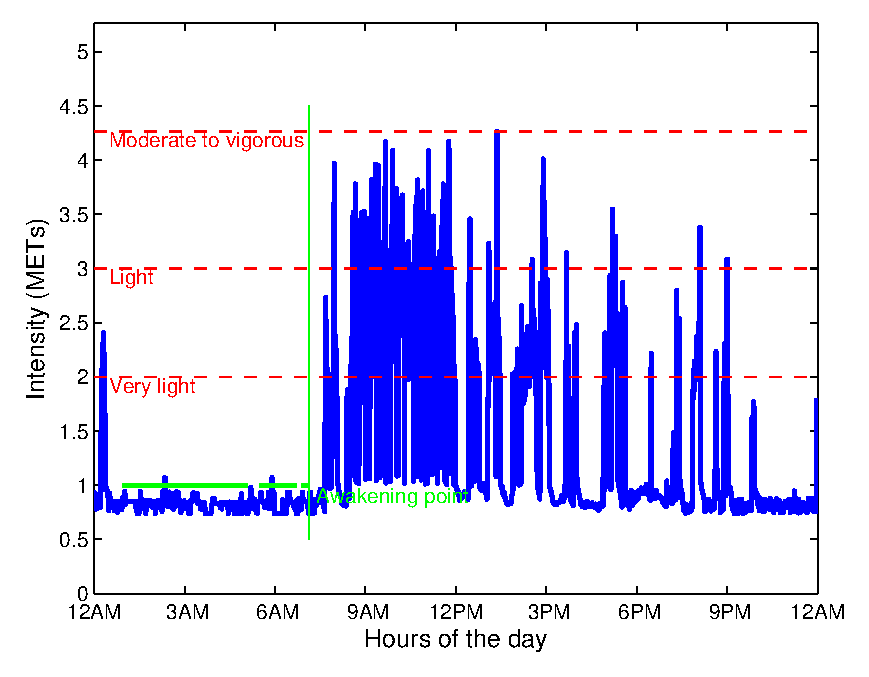
\includegraphics[width=.45\textwidth]{figure/eps/figure_1_1sub.eps}}}
%   \mbox{\subfloat[Quantization in intensity categories.]{\label{fig:1b} 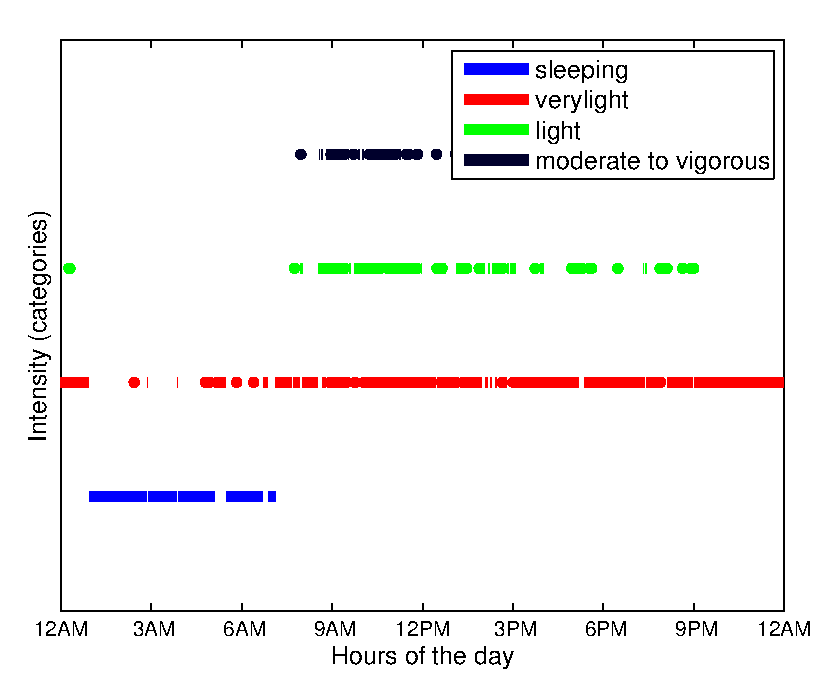
\includegraphics[width=.45\textwidth]{figure/eps/figure_2_1sub.eps}}}
%   \caption{Figure weekend-weekdays}\label{fig:1}
% \end{figure}
\begin{figure}[ht]
  \centering
  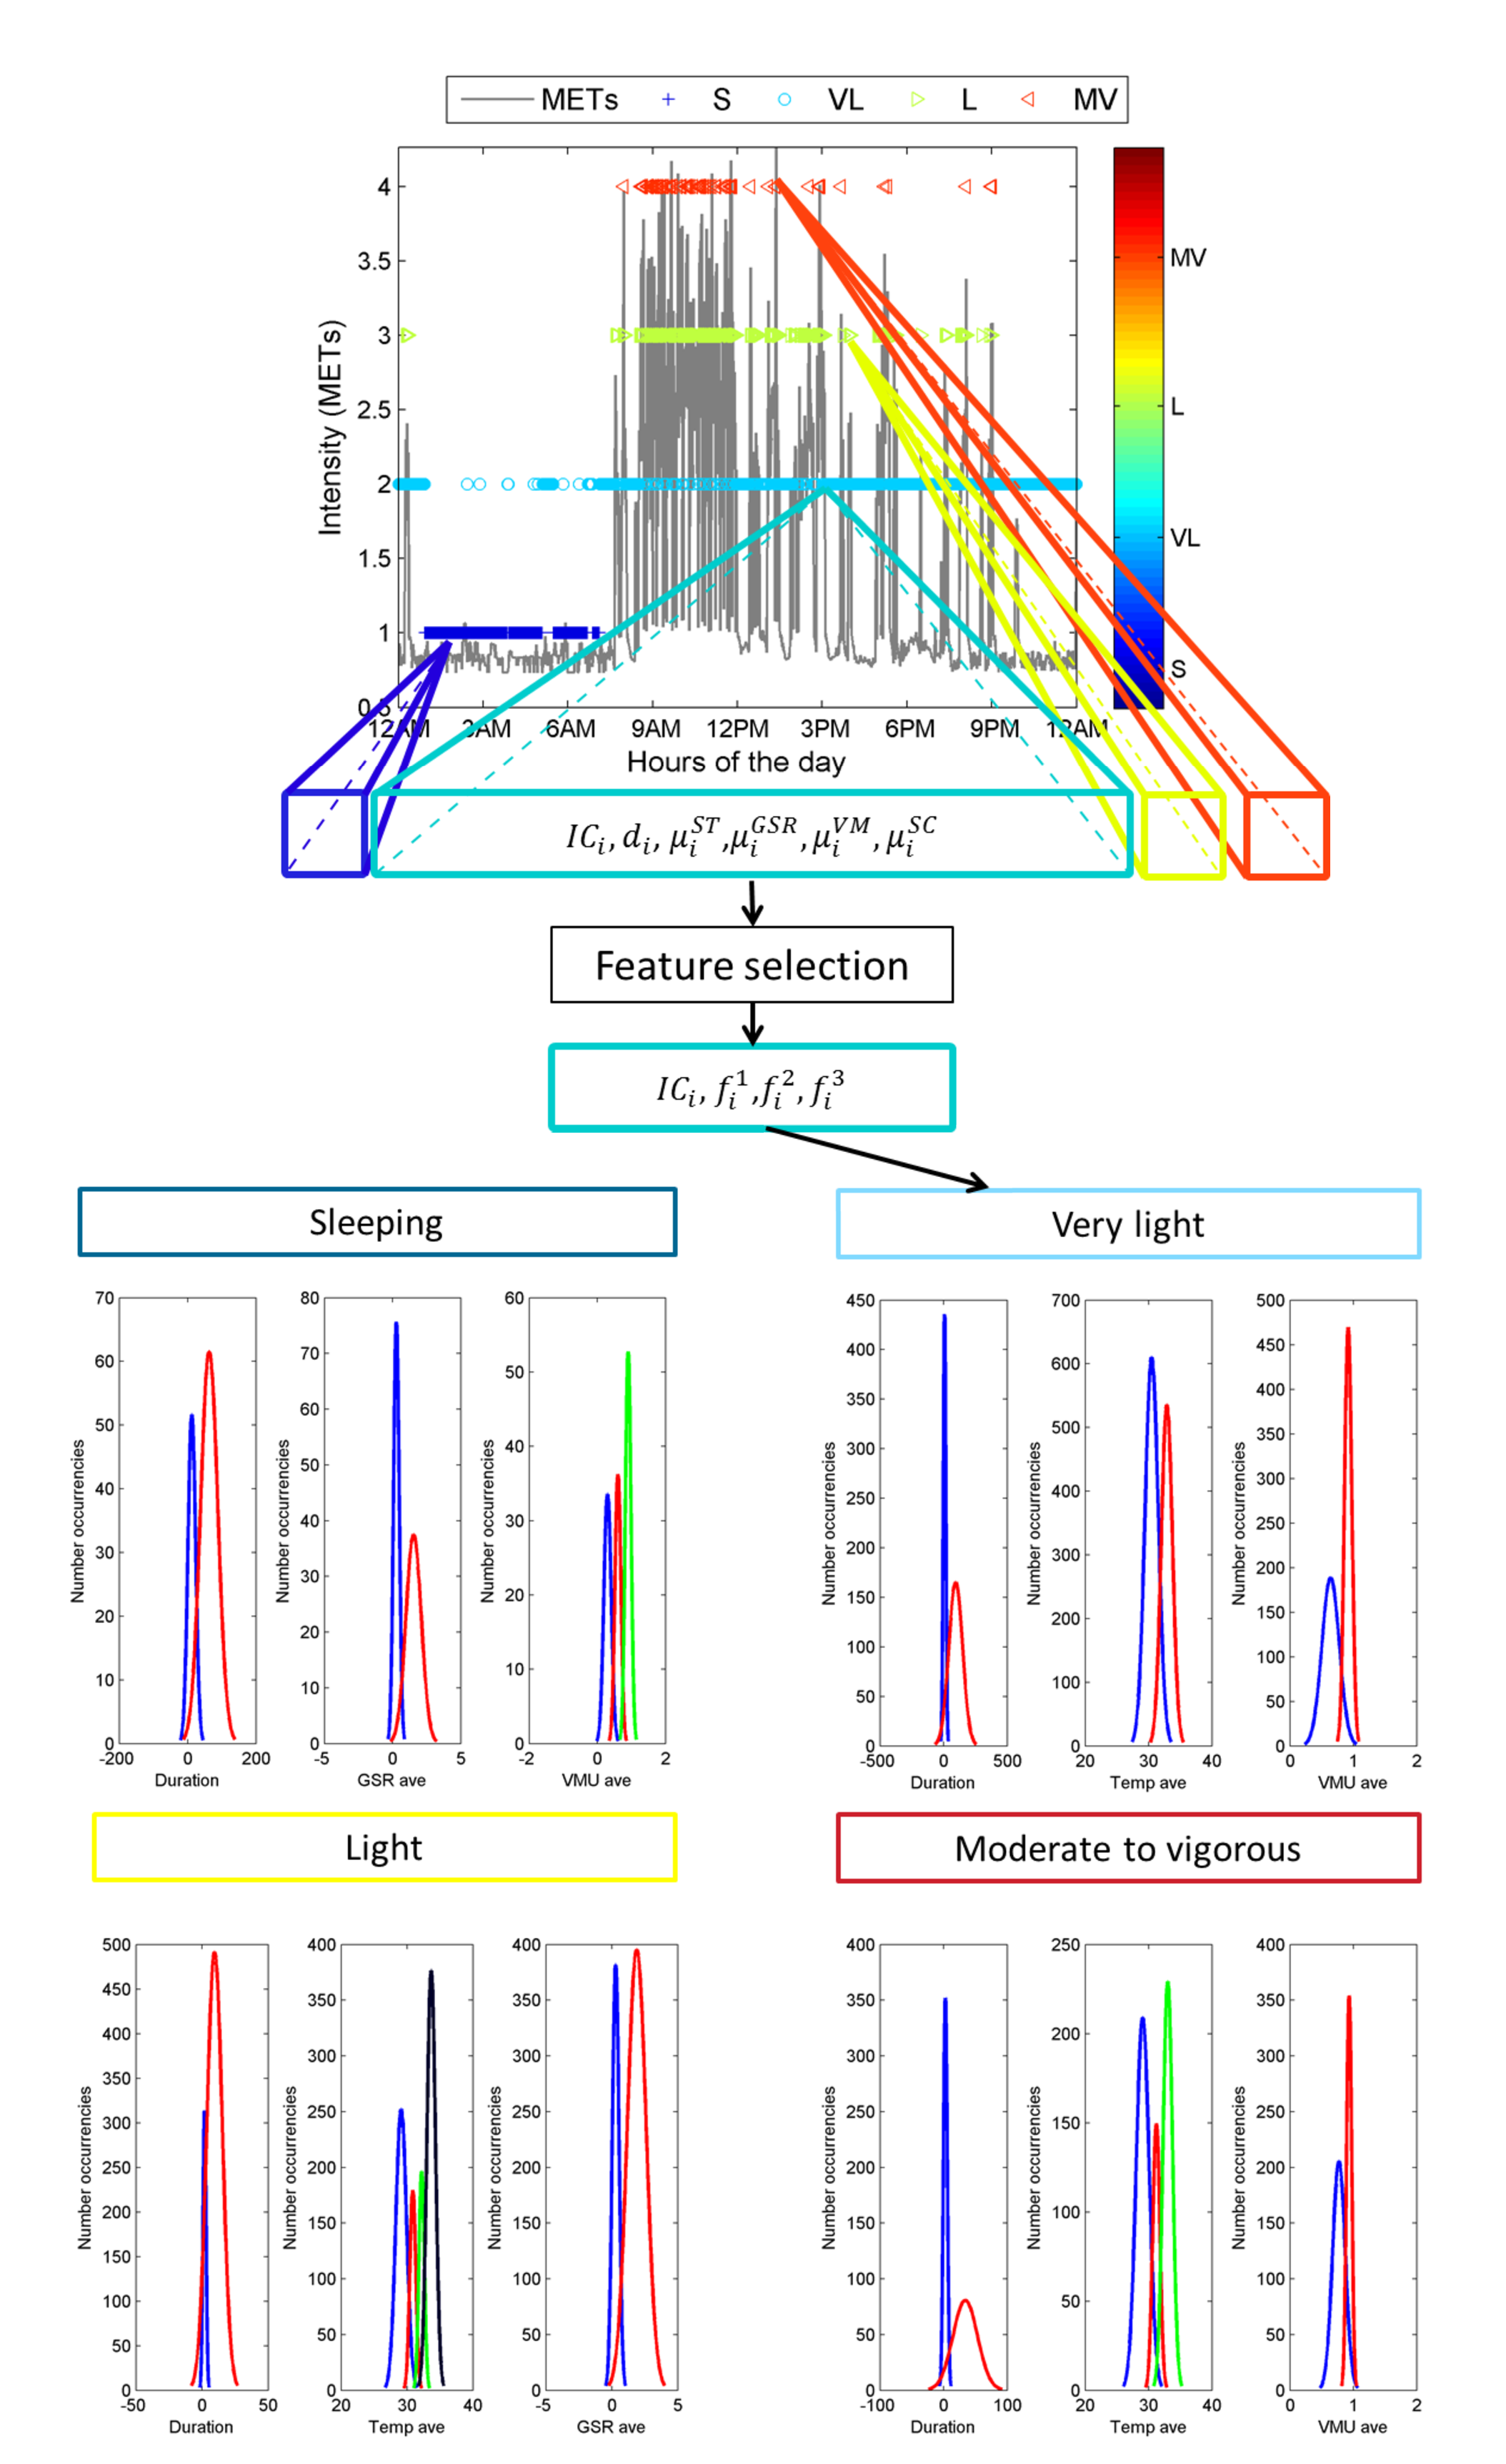
\includegraphics[width=.45\textwidth]{figure/eps/figure_11_together_mod_plus_arrow.eps}
  \caption[]{A continuous data stream representing METs value (grey line) is converted in bouts of PA intensity (blue=sleeping, ciano=verylight, green=light, and red=moderate to vigorous intensities). Features are computed within the bouts and the most relevant will be combine to create PA descriptors.}
  \label{fig:1}
\end{figure}
%%%%%%%%%%%%%%%%%%%%%%%%%%%%%%%%%%%%%%%%%%%%%%%%%%%%%%%%%%%%%%%%%%%%%%%%%%%
Consecutive minutes exhibiting the same $ICs$ are then grouped together in intensity bouts ($IB$) of variable duration ($d$). In each $IB$ we calculated the mean $\mu$ of $ST$, $GSR$, $VM$ and $SC$.
%\begin{itemize}
%\item Skin temperature ($u_{skt}$, $\sigma_{skt}$)
%\item Galvanic skin response ($u_{grs}$, $\sigma_{grs}$)
%\item Vector magnitude unit ($u_{vmu}$, $\sigma_{vmu}$)\\where $vmu=\sqrt{Acc_{x}^2+Acc_{y}^2}$ 
%\item Step counts ($u_{sc}$, $\sigma_{sc}$).
%\end{itemize}
The original sensor data stream is then represented by a series of intensity bouts where each bout is fully characterized by a 6-elements feature vector $\tilde{V}$ 
\begin{equation}
\tilde{V} = [IC, d, \mu_{ST}, \mu_{GSR}, \mu_{VM}, \mu_{SC}].
\end{equation}
Subsequently, for each intensity category ($S$, $VL$, $L$ and $VL$) the most relevant subset of features was selected such that the multi-cluster structure of the data can be best preserved. 
Features were selected using the Multi-Cluster Feature Selection (MCFS) that deploys spectral regression with \emph{l$_1$}-norm 
regularization in order to select features jointly instead of evaluating each feature independently~\cite{Cai_2010}. The feature vector $\tilde{V}$ can then be simplified according to
\begin{equation}
V = [IC, f_{1},f_{2},f_{3}].
\end{equation}
The reader might think about this step as a stemming procedure that removes redundant letters that might confuse the model.
The selected features $f_{j\in\{1,2,3\}}$ obviously might be different for each intensity and are shown in the bottom part of Fig.~\ref{fig:1}. 
\par To generate the vocabulary of words each of the selected features was first standardized and then mapped into a set of discrete levels using a K-means clustering algorithm. The algorithm automatically selects for each feature the number of levels $K^{f_{j}}$ (which could be interpreted as the letters of our words) in a way that the corresponding clustering results $L_{p\in\{1:K\}}$ are the most stable under small perturbations of the input dataset as described in~\cite{Luxburg_2010}.\\
Levels are sorted according to their mean value $\bar{L_{p}}$ in ascending order such that: first level ($L_{1}$) represents clusters with the smallest feature values and the last level ($L_{K}$) represents clusters with the highest feature values. 
Mean value and variance of the levels were stored and used to create the documents as described later in section~\ref{subsec:topicinf}. The vocabulary of terms was built by allowing all the possible combinations between levels sharing the same $IC$. 
%$N = K_{1} \cdot K_{2} \cdot K_{3}$ 
For the sleeping category, for example, the feature $f_{1}=d$, $f_{2}=\mu_{GSR}$ and $f_{3}=\mu_{VM}$ were selected and divided in $K^{f_{1}}=K^{f_{2}}=2$ and $K^{f_{3}}=3$ levels respectively.
The $N^{S}$ ($N^{S}=K^{f_{1}} \cdot K^{f_{2}} \cdot K^{f_{3}}$) terms of the vocabulary describing the sleeping intensity category ($t^{S}_{i\in\{1:N^{S}\}}$) are:
\begin{eqnarray}\label{eq:words}
t^{S}_{1}=\{L_{1}^{f_{1}}\_L_{1}^{f_{2}}\_L_{1}^{f_{3}}\}\nonumber\\
t^{S}_{2}=\{L_{1}^{f_{1}}\_L_{1}^{f_{2}}\_L_{2}^{f_{3}}\}\nonumber\\
...\nonumber\\
t^{S}_{12}=\{L_{2}^{f_{1}}\_L_{2}^{f_{2}}\_L_{3}^{f_{3}}\}\nonumber\\
\end{eqnarray}
The sum of terms across different activity levels is the total number of words.
%The feature selected for each $IC$, the $L_{p}$ levels for each feature are shown in~\ref{}. {\color{red}ADD TABLE WITH FEATURES, MEAN AND VARIANCE LEVELS.} 
In particular a total of 48 terms were created (12 for S, 8 for VL, 16 for L and 12 for MV intensity). Note that we did not need to specify the number of unique artificial words (vocabulary size) beforehand.
%Since rare words (defined as occurring less than twice in a document) do not affect much the inference process we did not consider them further in the analysis. 
As a last step frequent words (occurring at least in the 94\% of the documents) were removed because they will be placed by the model with high probability in all the topics. In other words they occur so frequently that they are more likely to obscure than facilitate a meaningful decomposition of the collection of documents. 
%{\color{red}SPECIFY WORDS THAT WERE REMOVED IN THE TABLE AND MAYBE PUT A FIGURE SHOWING THE FREQUENCY OF THE WORDS?.}

%The words used to create the set of topics are listed in table~\ref{table:Table 3}~\ref{table:Table 4}~\ref{table:Table 5}~\ref{table:Table 6}


%%%%%%%%%%%%%%%%%%%%%%%%%%%%	FIGURE FEATURE SELECTION		%%%%%%%%%%%%
%\newpage
%\begin{figure*}[ht]
%\centering
%  \mbox{\subfloat[Sleeping.]{\label{fig:5a} 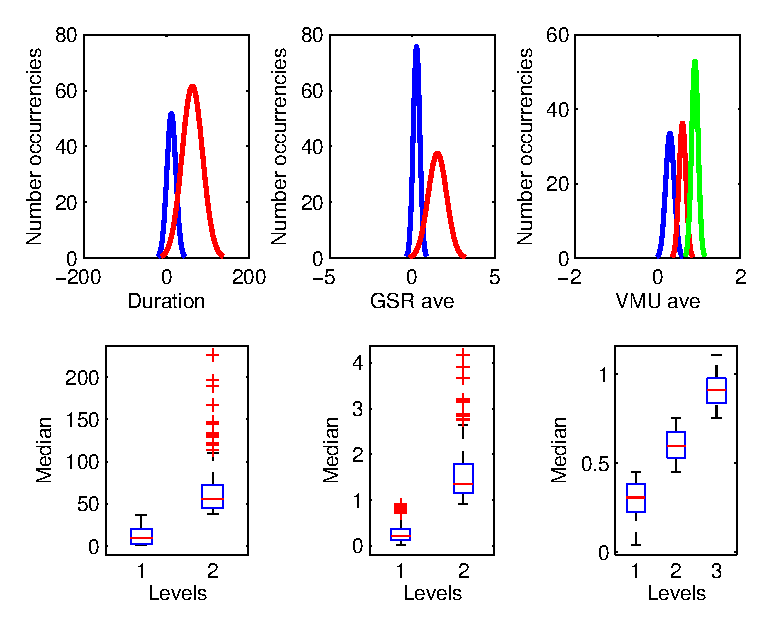
\includegraphics[width=.45\textwidth]{figure/eps/figure_5_sleeping.eps}}}
%  \mbox{\subfloat[Very light.]{\label{fig:5b} 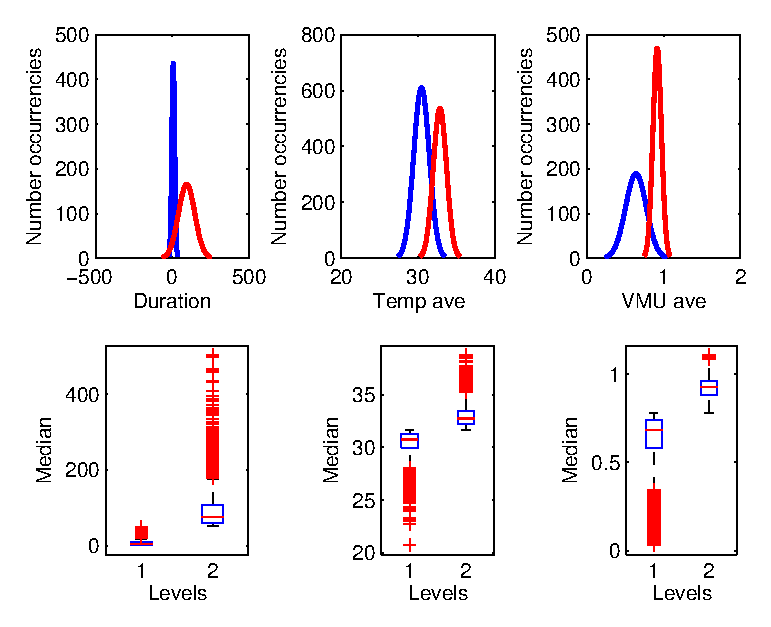
\includegraphics[width=.45\textwidth]{figure/eps/figure_5_verylight.eps}}}
%  \mbox{\subfloat[Light.]{\label{fig:5c} 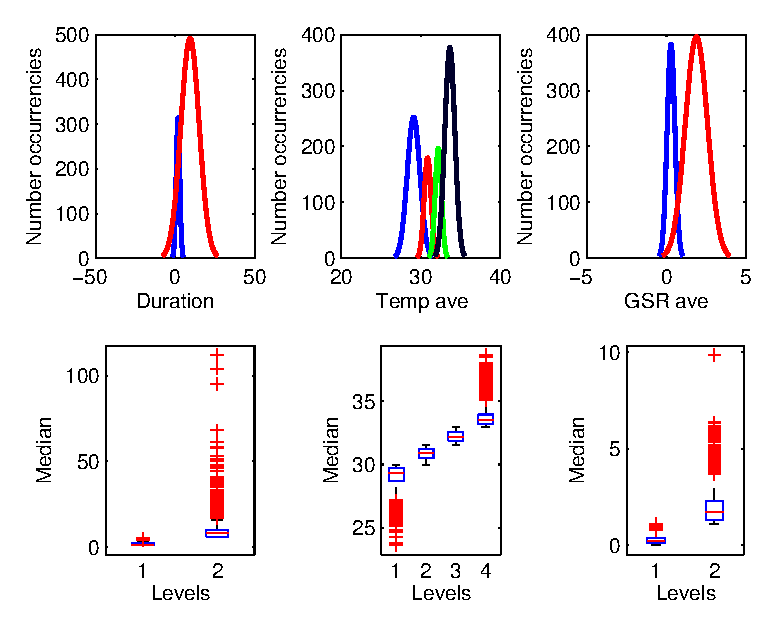
\includegraphics[width=.45\textwidth]{figure/eps/figure_5_light.eps}}}
%  \mbox{\subfloat[Moderate to vigorous.]{\label{fig:5d} 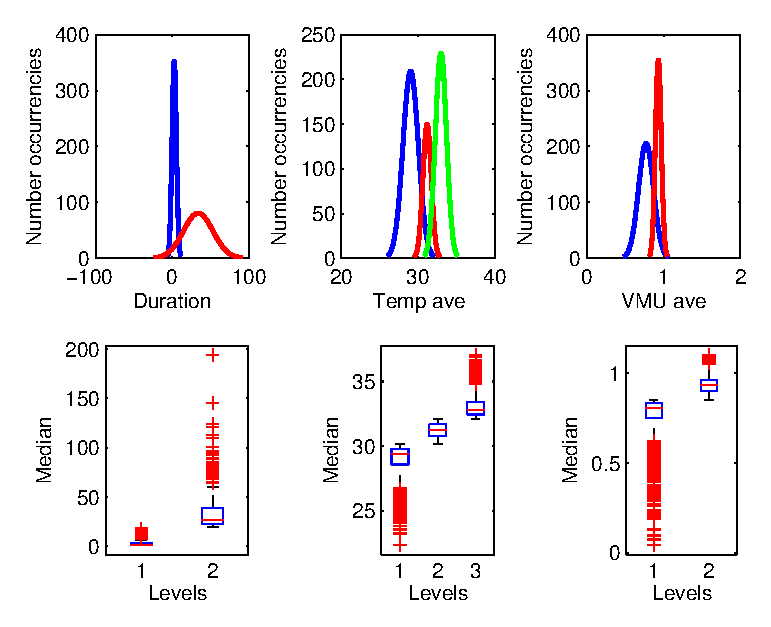
\includegraphics[width=.45\textwidth]{figure/eps/figure_5_MVPA.eps}}}
%\caption{Scatter plot selected features}\label{fig:5}
%\end{figure*}




%\newpage
%%%%%%%%%%%%%%%%%%%%%%%%%%%%	TABLE FEATURE PER CLUSTER	%%%%%%%%%%%%%%%%
%
%
%\begin{table}[H!]                                                                                             
%{\tiny
%\centering                                                                                                    
%\begin{tabular}{|c|c|c|c|c|c|c|c|c|c|}                                                                        
%\hline                                                                                                        
% & Dur & T ave & \textbf{GSR} ave & \textbf{VMU} ave & Step count ave & T std & GSR std & VMU std & \textbf{Step count std} \\
%\hline
%Word 1 & 29.69 & 33.31 & 0.39 & 0.55 & 0.40 & 0.23 & 0.03 & 0.08 & 1.31 \\
%\hline
%Word 2 & 29.30 & 33.14 & 0.28 & 0.87 & 0.00 & 0.21 & 0.01 & 0.02 & 0.01 \\
%\hline
%Word 3 & 30.48 & 33.26 & 0.27 & 0.42 & 0.00 & 0.24 & 0.01 & 0.04 & 0.01 \\
%\hline
%Word 4 & 30.87 & 33.67 & 1.54 & 0.62 & 0.00 & 0.23 & 0.06 & 0.03 & 0.02 \\
%\hline
%\end{tabular}
%\caption{Average values cluster variables after removing frequent words (sleeping)}                                                                             
%\label{table:Table 3} 
%}
%\end{table}       
%
%
%\begin{table}[H!]                                                                                             
%{\tiny
%\centering                                                                                                    
%\begin{tabular}{|c|c|c|c|c|c|c|c|c|c|}                                                                        
%\hline                                                                                                        
% & \textbf{Dur} & \textbf{T ave} & \textbf{GSR} ave & VMU ave & Step count ave & T std & GSR std & VMU std & Step count std \\
%\hline
%Word 1 & 14.20 & 32.76 & 1.75 & 0.87 & 1.86 & 0.12 & 0.06 & 0.06 & 2.69 \\
%\hline
%Word 2 & 108.00 & 32.42 & 0.34 & 0.84 & 0.84 & 0.39 & 0.04 & 0.11 & 2.74 \\
%\hline
%\end{tabular}
%\caption{Average values cluster variables after removing frequent words (very light)}                                                                            
%\label{table:Table 4}                                                                                         
%}
%\end{table}  
%
%
%\begin{table}[H!]                                                                                             
%{\tiny
%\centering                                                                                                    
%\begin{tabular}{|c|c|c|c|c|c|c|c|c|c|}                                                                        
%\hline                                                                                                        
% & \textbf{Dur} & T ave & \textbf{GSR ave} & VMU ave & Step count ave & T std & GSR std & VMU std & \textbf{Step count std} \\
%\hline
%Word 1 & 19.19 & 31.86 & 0.42 & 0.87 & 14.91 & 0.16 & 0.02 & 0.05 & 8.87 \\
%\hline
%Word 2 & 4.79 & 32.44 & 1.94 & 0.89 & 17.36 & 0.07 & 0.05 & 0.04 & 8.03 \\
%\hline
%Word 3 & 4.17 & 32.55 & 0.35 & 0.91 & 39.05 & 0.06 & 0.01 & 0.05 & 28.95 \\
%\hline
%Word 4 & 4.17 & 31.72 & 0.30 & 0.89 & 12.29 & 0.05 & 0.01 & 0.04 & 4.42 \\
%\hline
%Word 5 & 5.37 & 31.56 & 0.32 & 0.89 & 19.65 & 0.07 & 0.01 & 0.05 & 11.77 \\
%\hline
%\end{tabular}
%\caption{Average values cluster variables after removing frequent words (light)}                                                                                
%\label{table:Table 5}                                                                                         
%}
%\end{table}  
%
%
%\begin{table}[H!]                                                                                             
%\centering                                                                                                    
%{\tiny
%\begin{tabular}{|c|c|c|c|c|c|c|c|c|c|}                                                                        
%\hline                                                                                                        
% & Dur & T ave & \textbf{GSR} ave & VMU ave & \textbf{Step count ave} & \textbf{T std} & GSR std & VMU std & Step count std \\
%\hline
%Word 1 & 6.65 & 31.10 & 0.33 & 0.88 & 15.26 & 0.09 & 0.02 & 0.05 & 9.34 \\
%\hline
%Word 2 & 7.05 & 31.26 & 0.40 & 0.94 & 79.13 & 0.10 & 0.02 & 0.03 & 18.57 \\
%\hline
%Word 3 & 9.56 & 31.94 & 2.27 & 0.90 & 30.79 & 0.10 & 0.11 & 0.05 & 14.20 \\
%\hline
%Word 4 & 30.78 & 28.95 & 0.55 & 0.87 & 35.00 & 1.10 & 0.19 & 0.07 & 16.53 \\
%\hline
%\end{tabular}
%\caption{Average values cluster variables after removing frequent words (MVPA)}                                                                                 
%\label{table:Table 6}                                                                                         
%}
%\end{table}  
%
%%%%%%%%%%%%%%%%%%%%%%%%%%%%%%%%%%%%%%%%%%%%%%%%%%%%%%%%%%%%%%%%%%%%%%%%%%%%

\subsection{Topic discovery}
For topic discovery we used the LDA implementation of~\cite{Blei_2003} and we considered each day of assessment as a separate document.
%
%(1) An instance of the vocabulary was assigned to each $IB_{i}$ by associating the selected features of $V_{i}$ with their closest levels and then concatenating the 3 closest levels found.
%
Each $IB$ was mapped with an instance of the vocabulary by associating the selected features in $V$ with their closest levels and then concatenating the 3 closest levels found. 
%
%(3) For each $IC$ we assigned a discrete term of the vocabulary that minimizes the distances between the selected features and the levels. 
The distance for each bout between the feature point $f_{j}$  and all the levels $L_{p}$ are
%\begin{equation}\label{eq:distance}
%d_{i,p}({f^{j},L_{p}}) = \mid{f^{j}_{i}-\tilde{L}^{f^{j}}_{p}}\mid , \forall p=\{1,...,K^{f^{j}}\}.
%\end{equation}
\begin{equation}\label{eq:distance}
d_{p}({f_{j},L_{p}}) = \frac{\left|f_{j}-\bar{L}^{f_{j}}_{p}\right|}{\sigma_{p}} , \forall p=\{1,...,K^{f^{j}}\}.
\end{equation}
Once that a term of the vocabulary was assigned to each $IB$, documents were created constructing for each day a histogram of terms occurrences. 
We chose the number of topics ($T$) equal to 18 and set the hyperparameter $\alpha$ equal to 0.01 as in~\cite{Huynh_2008}. Hyperparameters are optimized iteratively
within a variational expectation maximization (EM) algorithm based on observed words from 18 randomly selected documents (6 healthy subjects, 6 COPD patients).
%The discovered topics are ordered within a document according to their variational posterior Dirichlets. Topics are presented as
%distributions over the vocabulary.
%\begin{equation}
%\log{p(w | z=k)}.
%\end{equation} 
%To evaluate the topic model we used the LDA implementation
%of [1], which includes an iterative optimization for topic
%model parameters ;  regarding model likelihood. The initial
%hyperparameter  was set to  = 0:01 as suggested by
%[4].

\subsection{Topic inference}\label{subsec:topicinf}
Once the topics are calculated, to know which one was active during the different parts of the day, we inferred documents composed by day segments. Differently from the documents used to discover the topics, each document represents a mixture of terms over a window of time $D$. We used sliding windows of 30 minutes as suggested in~\cite{Seiter_2014}. 
%We used sliding windows of 30 minutes with 90\% overlap as suggested in~\cite{Seiter_2014}. 
For each window we constructed a histogram of terms occurrences by mapping the bouts in $D$ to the words in the vocabulary giving soft assignments. For each feature point in $V$ we calculated the distances $d_{1...K^{f_{j}}}({f_{j},L_{p}})$ from the mean values of associated levels as in~(\ref{eq:distance}).
The distances were converted in weights according to
%\begin{eqnarray}
%w_{i,p}(f^{j},L_{p})=\frac{e^{-\frac{d_{i,p}}{\sigma_{p}}}}{\sum_{p=1}^{K^{f^{j}}} e^{-\frac{d_{i,p}}{\sigma_{p}}}}
%\end{eqnarray}
\begin{eqnarray}
w_{p}(f_{j},L_{p})=\frac{e^{-d_{p}}}{\sum_{p=1}^{K^{f_{j}}} e^{-d_{p}}}
\end{eqnarray}
Thus smaller distances imply higher weights and the weights for different levels of one selected feature sum up to one. 
%The parameter $\sigma$ controls how fast the weights decline for more distant clusters.
%or use the mahalanobis distance instead
We then concatenate the weights as we did in~(\ref{eq:words}) creating combination of weights, each of one assigned to the related term of the vocabulary. 
Summing up the weights of a specific term across the feature selected and dividing by the sum of the weights of all the terms we get values comprised between 0 and 1 that indicate the probability that the term appear in the document segment $D$. Weights of terms referring to other intensities will be set to 0.
Recalling the example with a sleeping bout we have 12 weights $G_{i}^{S}$
\begin{eqnarray}
G^{S}_{1}=\frac{w_{1}^{f_{1}}+w_{1}^{f_{2}}+w_{1}^{f_{3}}}{\sum{_{t=1}^{N^{S}}}G_{t}}\nonumber\\
%\{w_{i,1}^{f_{1}}\_w_{i,1}^{f_{2}}\_w_{i,1}^{f_{3}}\}\nonumber\\
...\nonumber\\
G^{S}_{2}=\frac{w_{1}^{f_{1}}+w_{1}^{f_{2}}+w_{2}^{f_{3}}}{\sum{_{t=1}^{N^{S}}}G_{t}}\nonumber\\
%w^{S}_{2}=\{w_{i,1}^{f_{1}}\_w_{i,1}^{f_{2}}\_w_{i,2}^{f_{3}}\}\nonumber\\
...\nonumber\\
G^{S}_{12}=\frac{w_{2}^{f_{1}}+w_{2}^{f_{2}}+w_{3}^{f_{3}}}{\sum{_{t=1}^{N^{S}}}G_{t}}\nonumber\\
%w^{S}_{12}=\{w_{i,2}^{f_{1}}\_w_{i,2}^{f_{2}}\_w_{i,3}^{f_{3}}\}\nonumber\\
\end{eqnarray}
We next use the weights associated to each term to construct documents of size $D$. More specifically, for each term we sum up the weights $W_{t}$ over a feature window of length $D$, and then generate $m_{W_{t}}$ instances of the term by multiplying the sum of this weights by the document length $D$ and rounding to the next integer. 
